\documentclass[12pt]{report}
\usepackage{graphicx}
\usepackage{relsize}
\usepackage{amsmath}
\usepackage[utf8]{inputenc}
\usepackage{graphicx}
\usepackage{mathpazo}
\usepackage{float}
\usepackage[hyphens]{url}
\usepackage[breaklinks]{hyperref}
\usepackage[utf8]{inputenc} % Required for inputting international characters
\usepackage[T1]{fontenc} % Output font encoding for international characters
\usepackage{appendix}
\usepackage{xcolor}
\usepackage{booktabs}
\newcommand{\tabitem}{~~\llap{\textbullet}~~}
\usepackage{listings}
\usepackage{outlines}
\usepackage{tabularx}
\usepackage{multirow, makecell}
\usepackage{svg}
\usepackage{subcaption}
\usepackage{verbatim}

%\usepackage[russian]{babel}

\definecolor{codegreen}{rgb}{0,0.6,0}
\definecolor{codegray}{rgb}{0.5,0.5,0.5}
\definecolor{codepurple}{rgb}{0.58,0,0.82}
\definecolor{backcolour}{rgb}{0.95,0.95,0.92}

\lstdefinestyle{mystyle}{
    backgroundcolor=\color{backcolour},   
    commentstyle=\color{codegreen},
    keywordstyle=\color{magenta},
    numberstyle=\tiny\color{codegray},
    stringstyle=\color{codepurple},
    basicstyle=\ttfamily\footnotesize,
    breakatwhitespace=false,         
    breaklines=true,                 
    captionpos=b,                    
    keepspaces=true,                 
    numbers=left,                    
    numbersep=5pt,                  
    showspaces=false,                
    showstringspaces=false,
    showtabs=false,                  
    tabsize=2
}

\lstset{
  aboveskip=1ex,
  backgroundcolor=\color{gray!25},
  basicstyle=\small\ttfamily,
  belowskip=1ex,
  breaklines=true,
  columns=fullflexible,
  framerule=0pt,
  framexrightmargin=0em,
  framexleftmargin=0em,
  numbers=left,
  numberstyle=\footnotesize\sffamily,
  tabsize=2,
  style=mystyle
}

%--------------
% CUSTOM EDITS
%-------------

%Make Chapter Title 1 Line
\usepackage{titlesec}
\titleformat{\chapter}[hang] 
{\normalfont\huge\bfseries}{\chaptertitlename\ \thechapter:}{1em}{} 

%\renewcommand\listoftables{List of Tables}
%\renewcommand\listoffigures{List of Figures & Illustrations}

\graphicspath{ {./Images/} }







\begin{document}
%\raggedright
%----------------------------------------------------------------------------------------
%	TITLE PAGE
%----------------------------------------------------------------------------------------

\begin{titlepage} % Suppresses displaying the page number on the title page and the subsequent page counts as page 1
	\newcommand{\HRule}{\rule{\linewidth}{0.5mm}} % Defines a new command for horizontal lines, change thickness here
	
	\center % Centre everything on the page
	
	%------------------------------------------------
	%	Headings
	%------------------------------------------------
	
	\textsc{\LARGE Wilfrid Laurier University}\\[1.5cm] % Main heading such as the name of your university/college
	
	\textsc{\Large Department of Mathematics}\\[0.5cm] % Major heading such as course name
	
	\textsc{\large MA695 - Major Research Project}\\[0.5cm] % Minor heading such as course title
	
	%------------------------------------------------
	%	Title
	%------------------------------------------------
	
	\HRule\\[0.4cm]
	
	{\huge\bfseries Enhancing Low-Resource Named Entity Recognition Results with Data Augmentation via Abstractive Summarization}\\[0.4cm] % Title of your document
	
	\HRule\\[1.5cm]
	
	%------------------------------------------------
	%	Author(s)
	%------------------------------------------------
	
	\begin{minipage}{0.4\textwidth}
		\begin{flushleft}
			\large
			\textit{Author}\\
			Douglas \textsc{Bowen}\\% Your name
		\end{flushleft}
	\end{minipage}
	~
	\begin{minipage}{0.4\textwidth}
		\begin{flushright}
			\large
			\textit{Supervisors:}\\
			Dr. Yang \textsc{Liu}\\
			Dr. Xu (Sunny) \textsc{Wang}\\
			\text{ }\\
			\textit{Second Readers:}\\
			Ilias S. \textsc{Kotsireas}
		\end{flushright}
	\end{minipage}
	
	% If you don't want a supervisor, uncomment the two lines below and comment the code above
	%{\large\textit{Author}}\\
	%John \textsc{Smith} % Your name
	
	%------------------------------------------------
	%	Date
	%------------------------------------------------
	
	\vfill\vfill\vfill % Position the date 3/4 down the remaining page
	
	{\large July 24th, 2022} % Date, change the \today to a set date if you want to be precise
	
	%------------------------------------------------
	%	Logo
	%------------------------------------------------
	
	\vfill\vfill\vfill
	
\includegraphics[width=0.2\textwidth]{laurier-crest-rev.jpg}\\[0.1cm] % Include a department/university logo - this will require the graphicx package
	 
	%----------------------------------------------------------------------------------------
	
	\vfill % Push the date up 1/4 of the remaining page
	
\end{titlepage}









% ABSTRACT SECTION STARTS
\begin{abstract}
    News and other articles can provide valuable info - but need to be read, analyzed, and processed. In the past, this was done manually and could be costly and time-consuming. In recent years, Natural Language Processing (NLP) has become mainstream in its ability to extract a variety of information from structured and unstructured text, without human intervention. This provides a much quicker and more cost-effective tool than manual labour.
    
    Named Entity Recognition (NER) is one such information extraction method, allowing for the classification of named entities to be made automatically. Due to its unique characteristics and the large variance in different domains, NER has been widely studied in the past few decades.
    
    For models to extract named entities from articles, a large amount of NER labelled data is required to learn from and sufficiently make predictions. However, finding data that is labelled can be challenging. Though some common tag sets and domains have plenty of data available to train on already that have been compiled by the public (e.g. Wikipedia, Twitter, News), custom NER tags and niche domains often have little to no data available, making training quite challenging. As a result, steps must be taken to create a large dataset from scratch or a small low-resource set. Data augmentation (DA) is a technique that attempts to alleviate this. Through various approaches, individuals can create artificial data to supplement the original and help increase NER model performance without the need for costly human data curation.
    
    This project examines various approaches to data augmentation in low-resource domains wherein artificially produced training data is required for decent model training. The dataset simulates a low-resource scenario for data augmentation, and a new generation approach using abstractive summarization is used to create sentences with completely new structures from the original data. 
    
    Techniques to create a sufficient sample set of augmented NE data include (but are not limited to) weighting source article sentences by entity count prior to shuffling, cutting sentences with no entities, and shuffling sentences randomly to create new samples.
    
    Results show that utilizing an abstractive summarization technique to augment data provides a significant boost over the original unaugmented data for low-resource data. Summary results are similar to paraphrased results, but lower than rules-based results. As the data size increases, the boost provided diminishes for all methods as expected.
    
\end{abstract}
% ABSTRACT SECTION ENDS


\section*{Acknowledgements}

    I would like to extend my sincere thanks to everyone who provided support during this project. Firstly, to my advisors Dr. Xu (Sunny) Wang and Dr. Yang Liu, for supporting my efforts and for providing their expertise as well as helping guide my research with valuable suggestions and insights. Secondly, to my colleagues Yanan Chen, Ian Fraser, Jason Lechter, and Herteg Kohar who worked with me, helped in researching, and provided support in tackling issues throughout the project. Lastly, I would also like to acknowledge the funding that was provided by the Natural Science and Engineering Research Council (NSERC), the MITACS Accelerate Program, and The Quantum Insider (TQI).
    
\newpage

\tableofcontents % TABLE OF CONTENTS (ONE LINE)

%TABLES/FIGURES
\listoftables
\listoffigures




%BEGIN FIRST CHAPTER, INTRODUCTION
\chapter{Introduction}
    In the digital age news comes out at an incredible rate. Be it live tweets, online articles, published research, or anything in-between, so much information is coming in at one time and has become impossible for humans to process it all.
    
    %The field of Quantum Technology has recently exploded and the amount of news released is growing immensely every day. However, Quantum Technology is also a field that requires extensive domain expertise and thus cannot be quickly understood, even by experts.
    
    In some domains (such as quantum technology), the amount of data has steadily increased with the number of news releases growing every day. Subsequently, information from these releases can often require domain expertise and thus cannot be quickly understood without sufficient background research.
    
    Given the timely and costly manual labour required to review and research for a proper understanding in these domains, along with the general size of training data required for NLP tasks, data augmentation (DA) is a growing field of research that aims to lessen said burden. DA utilizes a variety of techniques that create "new" artificially created data points from the original data. However, Named Entity Recognition (NER) is one such information extraction task that has more stringent requirements in both the structure of the data and the information required from models. For NER tasks, the structure of a sentence is considered and from it, words are designated either as an entity or not. The sequence of the sentence provides the information to designate an entity and is thus important to maintain. As a result, general DA techniques that have been developed for other tasks tend not to apply as well to NER ones due to the contextual requirements.
    
    This project aims to examine data augmentation techniques that can be utilized for NER models in low-resource domains. Though entity classifications are not complicated, the information surrounding them can be confusing for computers. Examining the following snippet from a quantum technology article, "demonstrating the early application of NISQ solutions to the energy sector", a model would likely consider NISQ to be a company rather than scientific acronym if it was not trained in the domain. An augmented version using generation could alter the sentence to the form "NISQ solutions demonstrated promising results within the energy sector" which is still coherent in structure as required by NER models and yet provides new sentence structure to learn on. By examining and applying DA techniques, the time and subsequent cost that arise from requiring individuals with sufficient expertise to provide labelled data can be reduced significantly. With this information, inferences and changes in the industry can be more readily tracked without constant monitoring.

    The new augmentation method being examined relies on generating abstractive summaries as a means of creating sentences with new structure as compared to the original source article. Furthermore, approaches are taken to attempt giving priority to entities in the generated sentences. By utilizing summarization models, the generated text will hopefully contain a proper coherent structure with entities from the original text that is sufficiently unique when compared to the other sentences from the original article. To compare the success of this approach, a baseline will be constructed using other researched methods that have been proven successful in augmenting NER sentences. These are discussed in detail in the literature review.
    
    The research performed here will highlight the performance of abstractive summarization as compared to the original dataset, as well as compared to baselines via rule-based approach and a paraphrasing generative method. Results show that performance of abstractive summarization is quite similar to that of paraphrasing, but below that of the rule-based approach for X-Small, Small, and Medium size batches while the Large batch size has similar performance for all three.
    
    The remainder of this thesis is organized in the following order: Chapter 2, which covers the literature review on relevant research done by others; Chapter 3, which provides background information on underlying mechanisms; Chapter 4, which discusses the specific approach to be taken; Chapter 5, which presents the results of the research; Chapter 6, which discusses potential further work; and Chapter 7, which summarizes the paper.





\chapter{Literature Review}
    This section will address the literature and published research currently available that makes use of data augmentation (DA) techniques on some Named Entity Recognition (NER) process. Though the focus is on utilizing DA for in-domain, low-resource data, the literature of utilizing DA for other purposes is also examined.
    
    \section{NER-Focused Approach}
        Though many DA techniques have been proposed for general NLP tasks, the application of these DA techniques is not always possible in the case of NER. This is due to the challenge that NER models present, wherein the labelling process is based on each individual token within sentences.
        
        Critical to understanding NER DA methods, it is important to familiarize oneself with the required structure for NER data. There are three primary points of importance: (1) The sentence of a structure, used to gain insight through learned patterns, (2) The words or "tokens" within a sentence that may or may not be entities, and (3) the associated BIO-labels, indicating either the (B)eginning/(I)nside of a named entity, or (O)utside, for non-entities. Of course, there is also the variety of named-entity categories (entity types) associated with the aforementioned labels, however these can be selected as one sees fit and are non-standard across NER tasks. As a result of these tags, techniques that might transform a token have to avoid also changing their labelling which presents a unique challenge for DA in NER tasks.
    
    \section{Rule-Based Approaches}
        
        The simplest approach is one that focused on tweaking traditional rules-based NLP approaches to DA so that they may be applied to NER situations~\cite{Rules}. Four underlying rules-based methods for augmenting NER data were constructed, for which combinations of these methods could also be utilized. Each of the following methods utilizes a probability distribution to determine whether or not the suggested transformation should take place on the specified token/segment. A success rate \textit{p} is utilized in the binomial distribution (specifically, the bernoulli distribution for \textit{n}=1 trial).
        
        \begin{itemize}
            \item The first method discussed is Label-Wise Token Replacement (LWTR)~\cite{Rules} wherein each token within a sentence is evaluated randomly for success or failure. If the randomly generated number outputs a success, the token is replaced with a randomly selected token designated with the same label. Otherwise, no replacement occurs and the next token is evaluated in the same way.
            
            \item The second method discussed is Synonym Replacement (SR)~\cite{Rules}. In a very similar method as to LWTR, each token within a sentence is evaluated randomly. In the case of SR however, if the randomly generated result indicates a success, the token is replaced with a synonym of itself. For synonyms that are multi-word, the associated label is applied in the standard B-Entity, I-Entity order.
            
            \item The third method discussed is Mention Replacement (MR)~\cite{Rules}. If a token is marked replacement, an entry with the same entity type is swapped into its place. The BIO-label for the new token being replaced should be maintained (i.e. the label should also be replaced).
            
            \item The final method discussed is substantially different from LWTR~\cite{Rules}, SR, and MR. Shuffle within Segment (SIS) evaluates each continuous segment of labels within a sentence randomly for success or not. In the case of success, the segment will be randomly shuffled to alter the order of tokens, but not labels.
        \end{itemize}
        
        Lastly, it is possible to use any combination/mixture of the above methods for a more comprehensive approach to data augmentation. Figure \ref{fig:rule_based_img} highlights these methods with an example provided by the original researchers.
        
        \begin{figure}[H]
            \centering
            \makebox[\textwidth]{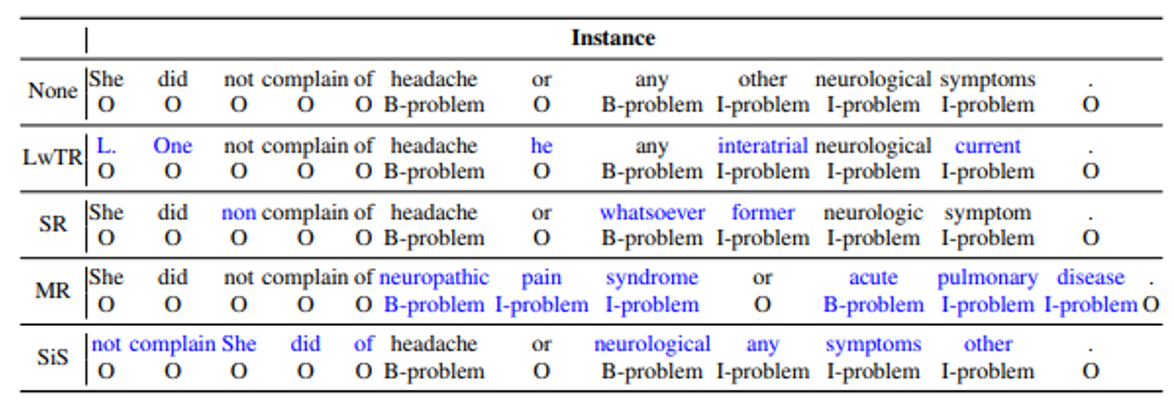
\includegraphics[scale=0.95]{Images/rule_based.png}}
            \caption{Rule-Based Method Examples~\cite{Rules}}
            \label{fig:rule_based_img} 
        \end{figure}
        
    \section{Basic Generation Approach}

        Another recent approach to augmenting NER data utilizes generational language models that are trained on linearized labelled sentences~\cite{Gen}. This method was applied to both supervised and semi-supervised data wherein both resulted in performances above baseline. Unlike the rules-based approach which simply applies adjustments to data without significantly altering them, generation-based approaches attempt to create sentences that have completely new structures with different words, contexts, phrases, etc., while still remaining coherent to the human eye. Thus the generated sentences still share similar patterns and trends to the original data that a model can find.
        \\\\
        Prior to utilizing a language model, sentences have tags added to the beginning and end of sentences, denoted as [BOS] and [EOS] respectively. Furthermore, named entities have their labels added in front of their respective tokens to linearize the sentence. After the completion of this process, a language model can be utilized. In this instance, a one-layer Long-Short Term Memory (LSTM) Recurrent Neural Network (RNN) is chosen as the language model. To train the generation model, each token is fed into the model in a linearized sentence order such that the first entry is [BOS] and the last entry is [EOS]. Each token then encounters a dropout layer, LSTM layer, another dropout later, and finally produces a prediction for the next token that should occur. With the trained model, synthetic data is generated by first feeding a [BOS] tag into the LSTM RNN, which then outputs a prediction. This prediction is then fed into the model as the next token in the sentence, and so on until sentence completion. This generated sentence is then de-linearized, with labels being added back into the proper order and [BOS]/[EOS] being removed.
        \\\\
        Another generation approach, albeit a bit more involved, is one that utilizes a Sequence-to-Sequence (Seq2Seq) Language Model to back-translate a sentence~\cite{Back}. As a simple overview, the process involves first splitting a sequence of tokens so as to break it into continuous label segments. Then, segments of 3 tokens or more that do not correspond to an entity type are fed into the model for translation from English to German and back again. The result of this back-translation is a sentence slightly different from the original in most case due to how each model handles the translation.
        
        
    \section{Cross-Domain Generation Approach}
        
        One method takes a different approach from the aforementioned methods. Wherein those methods focus on data augmentation in low-resource scenarios that are common in niche fields such as Quantum Technology, this approach attempts to leverage data from a high-resource domain and subsequently project it into the low-resource domain by utilizing semantics and patterns inherent to all text, even if textual patterns differ~\cite{Cross}. This approach builds off the work done in the generation approach.
        \\\\
        Similarly to the generation approach, this method begins by linearizing sentences, but then pairs a "source" domain sentence with a "target" domain sentence. Each sentence then has noise added through shuffling, dropouts, or masking. Once this is done, the domain-sentence pairs are fed into the model to output into the paired domain, which allows for the models to learn a "mapping" between domains.
    
    \section{Paraphrasing}
    
        A final method is the use of paraphrasing (expressing a sentence's meaning with different word structure) to augment NER data. A Bidirectional Encoder Representations from Transformers (BERT) model is utilized for entity recognition, while the underlying model utilized for the paraphrasing is not present in the published article. Researchers first replaced tokens with their respective entity tags (not "O" tags) and then performed both paraphrasing and back-translation on the sentence to generate newly augmented sentences. Both methods (paraphrasing vs. back-translation) were compared against one another, with paraphrasing proving successful at improving the BERT model at \textit{very} low resource data levels~\cite{Paraphrasing}.

\chapter{Background}
    This chapter provides a generalized overview of concepts not formally found in papers, but that are relevant to the research conducted henceforth.
    
    \section{Evaluation Metrics}
            \subsubsection{Precision, Recall, \& F1}
            These are standard metrics used for evaluating mistakes made by models. Precision measures the rate of false-positives, recall measures the rate of false-negatives, and F1 showcases the performance taking into account precision and recall trade-offs.
            
            \subsubsection{Recall-Oriented Understudy for Gisting Evaluation}
            More commonly known as "ROUGE", this is another important metric that will be used, albeit only in baseline construction and testing of the pre-trained Seq2Seq model. ROUGE evaluates the effectiveness of a summary or translation as compared to a human-produced reference.

    \section{Common Model Structure}
        Seq2Seq models are also commonly referred to as encoder-decoder models. Encoders receive inputs (for example, tokens within a sentence) and use said inputs to find relationships and acquire an "understanding" of the input. This understanding comes in the form of numerical outputs, which are then sent to the decoder and called "context vectors". Once encoding is complete, the context vectors along with a starting token are passed into a decoder. Decoders then read the context vector and starting token inputs and try to predict outputs, token by token. Figure \ref{fig:seq2seq} and \ref{fig:seq2seq1} display a very basic Seq2Seq overview. The encoder and decoder segments are in actuality often both built on recurrent neural networks, which are either Gated Recurrent Unit (GRU) or Long-Short Term Memory (LSTM) networks. However, this is not the case for transformers.
        
        \begin{figure}[H]
            \centering
            \makebox[\textwidth]{\includesvg[width = 425pt]{encoder_decoder.svg}}
            \caption{Basic Seq2Seq Model Architecture~\cite{HF_course}}
            \label{fig:seq2seq}
        \end{figure}
        
        \begin{figure}[H]
            \centering
            \makebox[\textwidth]{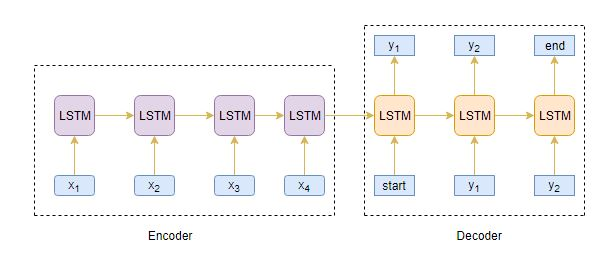
\includegraphics[width = 500pt]{encoder_decoder_detail.jpg}}
            \caption{Encoder-Decoder Details~\cite{HF_course}}
            \label{fig:seq2seq1}
        \end{figure}
    
    
    
    \section{Transformers}
        Transformers are built with "attention" in mind. Attention is a method wherein encoders and decoders are fed only the relevant inputs. To denote these inputs, inputs are assigned weightings where higher weights denote higher importance. These weightings are adjusted over time using feed-forward neural networks. Overall, transformers try to predict an output using only the important parts of the sentence, therefore giving a higher degree of "attention" to important input words over the others. The transformer process is very involved and thus more easily visualized as in Figure \ref{fig:seq2seq2}.
    \newpage
        \begin{figure}[H]
            \centering
            \makebox[\textwidth]{\includesvg[width = 800pt]{transformers.svg}}
            \caption{Transformer Encoder-Decoder Architecture ~\cite{HF_course}}
            \label{fig:seq2seq2}
        \end{figure}
    
    \newpage
    \section{Model Hyper-Parameter Choices}
    
        HuggingFace provides a strong API with a large array of customization choices~\cite{HF} for users to control. Part of these customization choices are the numerous parameters that can be tuned to impact a model's generation. This section will discuss the main parameters that are utilized to tweak generated outputs, as well as discuss parameters that can reduce repetition or increase entity inclusion rates. It should be noted that though there are many parameters to adjust, they often only have a small impact on the generated output.
        
        \textbf{Common Adjustments:}
        
        \begin{itemize}
            \item \textbf{Minimum \& Maximum Length:} Sets the minimum and maximum lengths that the generated output can be. While the maximum length is a hard cut-off, the minimum length is not always reached if there are no more suggested tokens for generation. Furthermore, setting a minimum length can also force the model to make longer generations, which is ideal for our goals.
            
            \item \textbf{Temperature:} A numerical input that increases or decreases the confidence a model has in what the most likely response is. A higher value makes the model less confident. For example, a model that has a low temperature examining the following sentence "The mouse ate some \_\_\_\_" might consider "Cheese" to be the correct word with 95\% confidence and 5\% confidence for "Pizza". If the temperature were set higher, it might begin to equalize the confidence wherein "Cheese" would drop to 75\% and "Pizza" rise to 25\%. As temperature rises higher, the rates would equalize further.
            
            \newpage
            
            \item \textbf{Greedy Searching:} This method selects the word with the highest probability, conditional on all prior words, as the next entry. This method is quite simple but can lead to poor and unvaried results as words with very high conditional probabilities can be skipped over if they're masked by earlier words with low probabilities. In Figure \ref{fig:greedy}, the starting word prior to generation is "The". As we follow along the lines or beams, we find that the next words could be "dog", "nice", or "car" with 40\%, 50\%, and 10\% probability respectively. And so when utilizing a greedy search, the highest probability is selected and the beams not selected are discarded.
            
            \begin{figure}[H]
            \begin{center}
            \makebox[\textwidth]{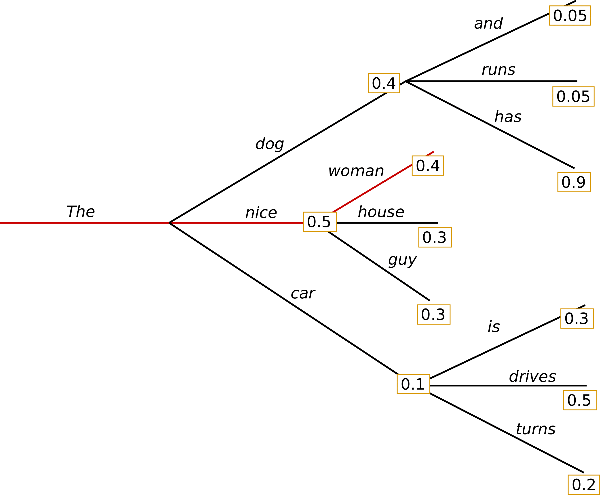
\includegraphics[width=14cm]{greedy_search.png}}
            \caption{Greedy Search Generation ~\cite{HF}}
            \label{fig:greedy}
            \end{center}
            \end{figure}
            
            \newpage
            
            \item \textbf{Beam Searching:} Beam searching provides a solution to the masking that occurs when utilizing a greedy search. Though it is more costly, this method keeps track of the probabilities for \textit{n}-beams and then selects the words giving the highest probability. Figure \ref{fig:beam} is a simple repeat of the one from the greedy searching section, but now has an additional line (going upwards instead of straight ahead after "The"). If the number of beams in a beam search were set to 2, the generative model would explore both the highest and second highest probability beams, in this case "Nice" and "Dog". At the next time step, it would then find the sequence "The dog has" to have an overall higher probability and thus would select this beam instead of the original, "The nice woman".
            
            \begin{figure}[H]
            \centering
            \makebox[\textwidth]{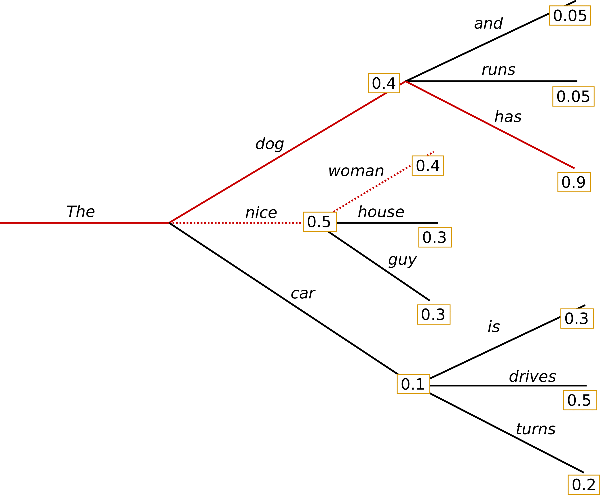
\includegraphics[width=14cm]{beam_search.png}}
            \caption{Beam Search Generation ~\cite{HF}}
            \label{fig:beam}
            \end{figure}
            
            \newpage
            
            \item \textbf{Sampling:} This method randomly selects the next word based on the conditional probability distribution of the prior words.
            \begin{itemize}
                \item \textbf{Top-K Sampling:} By utilizing Top-K sampling, the \textit{k} most likely words are selected, while the rest of the potential words are removed, thus changing the probability distribution of the remaining \textit{k} words.
                \item \textbf{Top-P (Nucleus) Sampling:} In a very similar process to Top-K sampling, Top-P or "Nucleus" sampling selects the smallest group of words whose total probability exceeds some rate \textit{p}. Thus it provides a more dynamic approach as compared to Top-K.
            
            \begin{figure}[H]
            \centering
            \begin{subfigure}[b]{0.75\textwidth}
               \makebox[\textwidth]{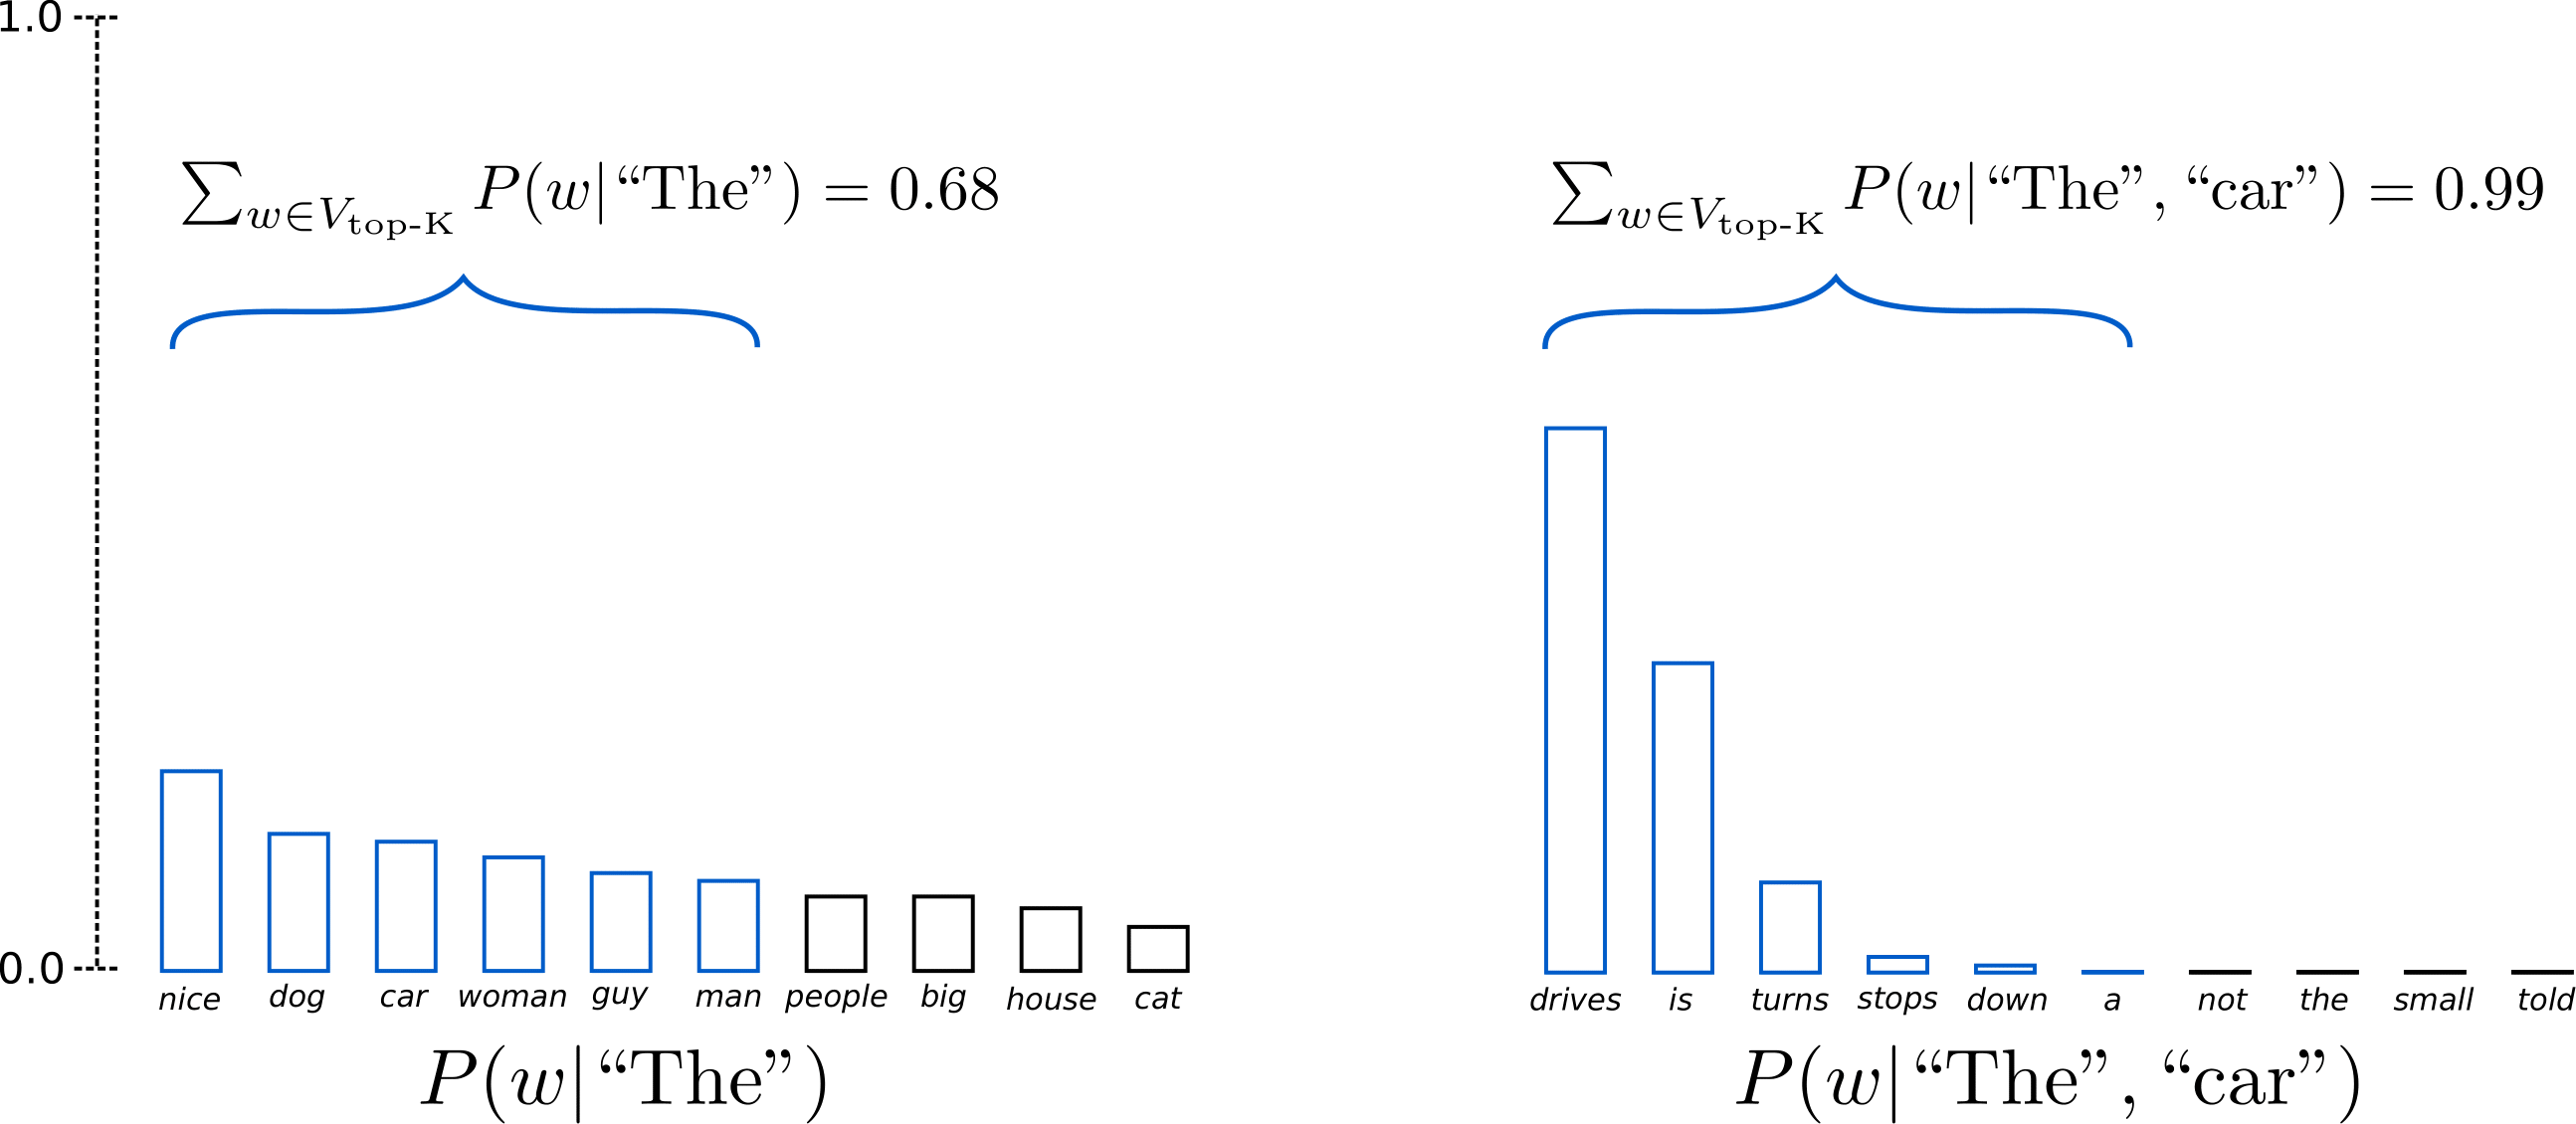
\includegraphics[width=1.1\linewidth]{Images/top_k_sampling.png}}
               \caption{Top-K Sampling}
               %\label{fig:Ng1} 
            \end{subfigure}
            
            \begin{subfigure}[b]{0.75\textwidth}
               \makebox[\textwidth]{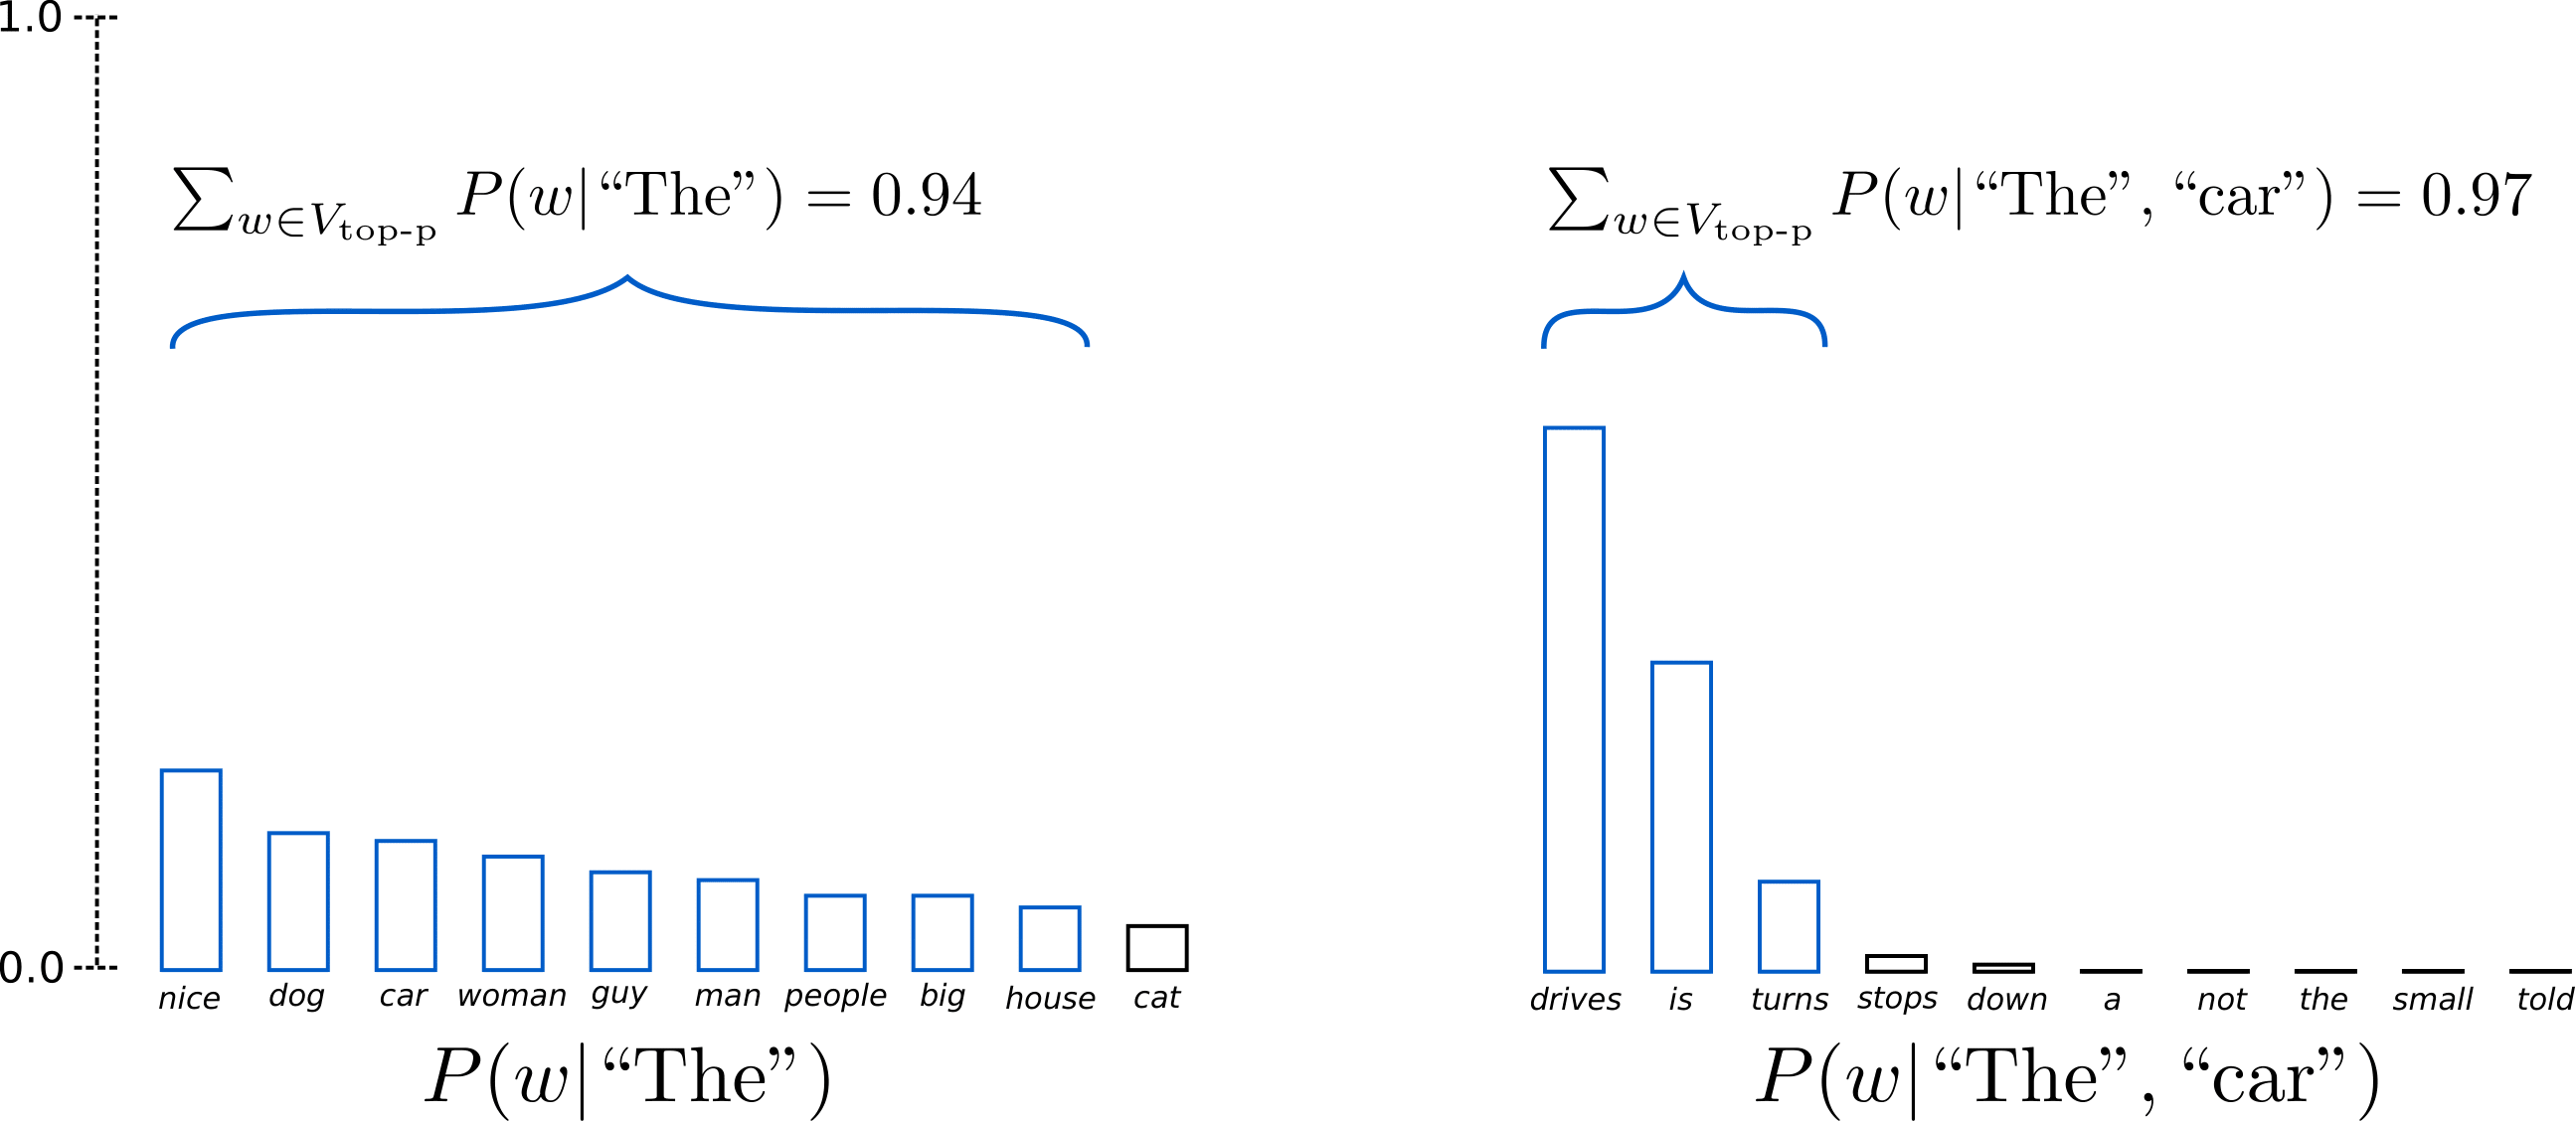
\includegraphics[width=1.1\linewidth]{Images/top_p_sampling.png}}
               \caption{Top-P Sampling}
               %\label{fig:Ng2}
            \end{subfigure}
            \caption{Sampling Methods ~\cite{HF}}
            \end{figure}
            
            \end{itemize}
        \end{itemize}
        
        \textbf{Repetition Solutions:}
        
        \begin{itemize}
            \item \textbf{Repetition Penalty:} One common issue with generated outputs is that tokens can tend to repeat themselves. As a quick overview, setting a penalty value reduces the value given to tokens that have already appeared. There is also a setting that can prevent \textit{n}-gram repetition by preventing any outputs that would have an \textit{n}-gram appear twice.
        \end{itemize}
        
 
    \section{Known Abstractive Summarization Issues}
        This section will provide some background on known issues with abstractive summarization generation, with examples from the dataset used presented. There are two issues that are well-known and well-researched in the NLP field, and various solutions have been proposed to mitigate them. One of the common issues in text generation is repetitive outputs, while the other is that generated text can create new entities that were not present in the original text and can even go on tangents related to these entities. Due to the use of pre-trained models for this project which prevents the altering of the underlying Seq2Seq encoder-decoder structure, some of the researched solutions could not be implemented, but are still discussed.
        
         As an example used in this research, Table \ref{tab:degeneration} displays one of the original articles from the WikiGold dataset~\cite{data_source} and two of the subsequent summarizations provided by the selected summarization model. Though the cases with repetition and entity hallucination are not necessarily frequent, different paragraph structures and hyper-parameter configurations can influence rates of occurrence.
         
         \begin{table}[H]
            \begin{center}
            \begin{tabular}{|l|p{9cm}|}\hline
                
                \textbf{Type} & \textbf{Output}\\\hline
                
                Original & 010 is the tenth album from Japanese Punk Techno band The Mad Capsule Markets . This album proved to be more commercial and more techno-based than Osc-Dis , with heavily synthesized songs like Introduction 010 and Come . Founding member Kojima Minoru played guitar on Good Day , and Wardanceis cover of a song by UK post punk industrial band Killing Joke . XXX can of This had a different meaning , and most people did n't understand what the song was about . it was later explained that the song was about Cannabis ( ' can of this ' sounding like Cannabis when said faster ) it is uncertain if they were told to change the lyric like they did on P.O.P and HUMANITY . UK Edition came with the OSC-DIS video , and most of the tracks were re-engineered .
\\\hline
                Repetition Loop & Japanese Punk Techno band The Mad Capsule Markets' second album Osc-Dis was met with a lot of controversy after the band changed the lyrics of their song XXX can of This to make it sound more like \color{blue} XXX can of This, make it sound more like XXX can of This, make it sound more like XXX can of This, make it sound more like XXX can of This\\\hline
                
                Entity Hallucination & Japanese Punk Techno band The Mad Capsule Markets have released their second album.010 in the UK, following the success of their first album Osc-Dis, which was released in the UK and \color{red}Ireland\color{black}\ in May of this year and became one of the best-selling albums of all time in \color{red}Ireland\color{black}.\\\hline
                
            
            \end{tabular}
            \end{center}
            \caption{Example of Summary Degeneration}
            \label{tab:degeneration}
            \end{table}
         
         \newpage
        
        In the paper "The Curious Case of Neural Text \textit{De}Generation"~\cite{Degen}, the authors explored hyper-parameter tuning options and their impact on both repetition and entity hallucination rates. While this paper was for sequential text generation as opposed to abstractive summarization, it still provides valuable insights.
        
        \subsubsection{Repetition Loops}
            In a further expansion on the paper by Holtzman et al. exploring text degeneration, the likelihood objective function was examined to determine if it had an impact on degeneration~\cite{Anon}. After examination, it was found that the likelihood function was giving too much weight to generated outputs that contained repetition. To solve this issue, researchers adjusted the likelihood objective function to penalize unlikely tokens further than it otherwise might have at both a sequence and token level.
            
            Furthermore, though the above techniques were tested on sequential text generation, this method of "unlikelihood" training was also extended for abstractive summarization~\cite{unlik}, with some modifications made. As a baseline without any tweaks, the unlikelihood method boosted ROUGE scores and reduced repetition. The key modification applied to further boost scores and reduce repetition used a variation on a coverage mechanism that penalized the model if the decoder's cross attention mechanic examines the same token multiple times. This variation acted on a token level, wherein the model is penalized for giving high probabilities to the same tokens multiple times.
            
        \subsubsection{Entity Hallucination/Factual Consistency}
            One such approach to handling entity hallucination hypothesized that the issue of entity hallucination is embedded within the training dataset. The researchers~\cite{hallucinate} proposed three new metrics to quantify if entities are consistent across both source and generated texts. 
            
            \begin{itemize}
                \item Precision-Source or Prec(S) = N(G $\cap$ S) / N(G)\\ Where N refers to the entity set for the source document (S) and generated summary (G). This metric examines how many entities from the generated summary are a part of the source document.
                \item Precision-Target or Prec(T) = N(G $\cap$ T) / N(G)\\ Where T refers to the human-made summary. This metric examines how many entities from the generated summary are a part of the human-made summary.
                \item Recall-Target or Recall(T) = N(G $\cap$ T) / N(T)\\ This metric examines how many entries from the human-made summary are \textit{not} present in the generated summary.
            \end{itemize}
            
            To mitigate entity hallucination, these metrics were utilized to subsequently filter out the dataset based on specific precision-recall thresholds. Specifically, if entities within the generated summary were not present in the source doc, the sentence in the summary is removed. If the summary is only one sentence, then the source document-human summary pair is entirely removed from the training data.
            
            Along with this data filtration method was a proposed change to encoder structure, wherein the encoder is trained to classify summary-"worthy" entities that are in the source document and human summary. The filtering of data combined with summary-"worthy" entity classification resulted in significant improvements in curbing entity hallucination.
            
            As the goal of this research is creating augmented data for named entity recognition, hallucination in summary outputs is un-ideal unless a method can be found to properly tag these newly added entities. Though this method was successful in reducing hallucination, it requires a training set with both source document and human-made summary. Unfortunately, no dataset exists that has (a) entity tags (b) source articles, and (c) human-made summaries of the articles. As a result, this method could not be employed. In an attempt to still mitigate the issue of entity hallucination, ROUGE score filtering is utilized and discussed in more detail in the Methodology chapter.


\chapter{Methodology}
    The methodology section aims to highlight the approach that will be taken stemming from the aforementioned methods and information discussed in the literature review and background sections. Some of these reviewed methods will serve as a baseline for comparison to the new approach examined. While rules-based data augmentation approaches have been fairly well studied, even within the NER field where the task is somewhat more challenging, generative data augmentation approaches have significantly less exposure and testing.
    
    \section{Proposed Summary Generation Approach}
        There are two types of summarization methods, these being extractive and abstractive. Extractive summarization is a method wherein each sentence within the overall text is evaluated for importance. These sentences are then compared amongst one another, at which point only the subset of sentences classified as important are used to construct a summary. Meanwhile, abstractive summarization evaluates the text and then generates a brand new summary, both taking portions from sentences as well as reorganizing, changing phrases, and adding/removing words.
        \\\\
        Since the goal of DA is to artificially construct \textit{new} sentences, extractive summarization provides no benefit. Any summary constructed would be a combination of sentences taken verbatim from the original data. Thus, we consider abstractive summarization for this project.
    \newpage
    \section{Overview of Process Pipeline}
        This section will quickly outline the steps to the process of generating sufficient abstractive summaries for data augmentation and subsequent testing. Section 4.3 through to Chapter 5 will go into more detail.
        
        \begin{enumerate}
            \item Pre-Trained Model
            \begin{enumerate}
                \item Abstractive Summary Models
                \item Named Entity Recognition Models
            \end{enumerate}

            \item Source Data Adjustments
            \begin{enumerate}
                \item Tag Linearization
                \item Tag Replacement Variants
                \item Named Entity Weighted Order
                \item Article Stemming
                \item Shuffling
                \item ROUGE Scoring
            \end{enumerate}
            \item Train-Test Splitting
            \item Model Training
            \item Model Evaluation and Comparison
            
        \end{enumerate}
    
    \section{Models for Abstractive Summarization}
        For summarization, there are currently 4 well-known options that can provide abstractive outputs (as opposed to extractive). These are:
            
        \begin{itemize}
            \item BART~\cite{BART}
            \item T5~\cite{T5}
            \item GPT-2~\cite{GPT2}
            \item PEGASUS (X-Sum Variant)~\cite{PEGASUS}
        \end{itemize}
        
        Of the above models, BART and T5 are Seq-2-Seq structured transformers, while GPT-2 is a decoder and PEGASUS has an underlying T5 model but was trained on data specifically for abstractive summarization. BART, T5, and GPT-2 can be utilized for text generation, translation, Q\&A, and abstractive summarization, among other things, while PEGASUS is geared more towards only abstractive summarization. The following sections briefly highlight the unique differences in models.
        
        \subsubsection{BART}
        The BART transformer structure was created by Facebook. The structure is an expansion on BERT, which at its core is a bi-directional encoder which was trained via masked language modelling. BART furthers this by adding in an autoregressive decoder to provide further functionality over BERT and access to standard encoder-decoder tasks. Training of the model first corrupted source text via noising function and then learned to reconstruct the corrupted text as close to source-level as possible.
        
        \subsubsection{T5}
        The T5 transformer structure is very similar to BART and was created by Google and released within the same week that BART was. It was also an expansion from BERT and thus has the same bi-directional encoder as BART, and further adds its own auto-regressive decoder. The primary differences in T5 and BART are the structure of layers within the decoder. One other slight difference is that the training method used by T5 is no longer corrupt/fill-in-the-blank but instead has a mix of variations used to train for different tasks.
        
        \subsubsection{GPT-2}
        GPT-2 was created by Open-AI and is a transformer structure comprised of only an autoregressive decoder. Training for GPT-2 occurred on web-texts, wherein it attempted to predict new tokens with only information of the prior ones given to it. The decoder method is similar to T5 and BART, but the actual structure of the model is different. Due to lack of support via HuggingFace for GPT-2 summarization, this model was not examined in the paper.
        
        \subsubsection{PEGASUS}
        PEGASUS was created by Google and based off the original T5 Seq2Seq transformer structure. Its goal was to fix other models' weaknesses in abstractive summarization generation. PEGASUS pre-trains the Seq2Seq model on a large text corpus wherein important sentences get removed/ masked from the input source and then generated utilizing the remaining sentences. As a result, this pre-trained model is quite strong at summarization specifically, but cannot be utilized as well for other Seq2Seq tasks.
        
        \subsubsection{Final Decision}
        Based on the training information for the above models, PEGASUS seems an ideal choice. To quantitatively verify this, a small sample of 25 articles from the WikiGold dataset were passed into all three models (BART, T5, PEGASUS) simultaneously, with each model using the same configuration of hyper-parameters. The output of each model was then examined by human eye for sentence structure and fidelity. The ideal (or "sufficient", these two words may be used interchangeably) output was one that was coherent, stayed mostly faithful to the original article, and also provided a new structure that was not simply re-utilizing a sentence directly from the article. Sufficient length was also a factor. Multiple hyper-parameter combinations were examined, after which point it became clear that the PEGASUS X-Sum model (herein referred to simply as PEGASUS) was able to provide the best results consistently (as seen in Table \ref{tab:verify_sum}. The other models tended to do one of three things most frequently:
        
        \begin{enumerate}
            \item Provide frequent incoherent, or repetitive outputs
            \item Provide extractive (or near-extractive) outputs as opposed to abstractive ones
            \item Provide excessively short outputs (\~3-7 words maximum, even for articles that were 300+ words).
        \end{enumerate}
        
        On the other hand, the PEGASUS model tended to provide outputs that were often coherent, of significant length (long or multiple sentences), and sufficiently unique from the sentences within articles.
        
        As a result, the PEGASUS model was selected for this research. After this selection, other variants of the PEGASUS model were also examined (such as those tuned specifically on CNN Daily Mail and WikiHow datasets), but the X-Sum variant proved most consistent. Table~\ref{tab:verify_sum} displays parameter settings by model and generated output issue rates on 25 articles.
        
        \begin{table}[H]
            \begin{center}
            \resizebox{\textwidth}{!}{%
            \begin{tabular}{|c|c|c|c|c|c|c|}
                 \hline
                 \textbf{Parameters} & \textbf{Model} & \textbf{Satisfactory} & \textbf{Extractive} & \textbf{Repetitive} & \textbf{Incoherent} & \textbf{Hallucination}    \\
                 \hline
                 \multirowcell{3}{Default}&
                 BART & 0/25 & 19/25 & 0/25 & 6/25&0/25\\&
                 T5 & 1/25 & 19/25 & 0/25 & 5/25&0/25\\&
                 %GPT-2 & ? & ? & ? & ?\\&
                 PEGASUS & 17/25 & 7/25 & 0/25 & 1/25 &0/25\\\cline{2-6}
                \hline
                \multirowcell{3}{MinLength=Article}&
                 BART & 0/25 & 22/25 & 0/25 & 3/25 & 0/25\\&
                 T5 & 1/25 & 22/25 & 0/25 & 2/25 & 0/25\\&
                 %GPT-2 & ? & ? & ? & ?\\&
                 PEGASUS & 18/25 & 0/25 & 5/25 & 0/25 & 2/25\\\cline{2-6}
                \hline
                \multirowcell{3}{MinLength=Article\\Top P=0.9}&
                 BART & 0/25 & 22/25 & 0/25 & 3/25 & 0/25\\&
                 T5 & 0/25 & 24/25 & 0/25 & 1/25 & 0/25\\&
                 %GPT-2 & ? & ? & ? & ?\\&
                 PEGASUS & 11/25 & 0/25 & 6/25 & 0/25 & 8/25\\\cline{2-6}
                \hline
                \multirowcell{3}{MinLength=Article\\Num Beams=32}&
                 BART & 0/25 & 22/25 & 0/25 & 3/25 & 0/25\\&
                 T5 & 0/25 & 23/25 & 0/25 & 2/25 & 0/25\\&
                 %GPT-2 & ? & ? & ? & ?\\&
                 PEGASUS & 17/25 & 0/25 & 6/25 & 0/25 & 2/25\\\cline{2-6}
                \hline
                \multirowcell{3}{MinLength=Article\\Num Beams=32\\RepetitionPenalty=2.0}&
                 BART & 0/25 & 22/25 & 0/25 & 3/25 & 0/25\\&
                 T5 & 0/25 & 23/25 & 0/25 & 2/25 & 0/25\\&
                 %GPT-2 & ? & ? & ? & ?\\&
                 PEGASUS & 17/25 & 0/25 & 4/25 & 0/25 & 4/25\\\cline{2-6}
                \hline
            \end{tabular}}
            \end{center}
            \caption{Summary Output Success Rates}
            \label{tab:verify_sum}
            \end{table}
        
        Clearly, PEGASUS heavily outperforms the T5 and BART models. As for the impact of parameters on the PEGASUS model, the minimum length being set to the article length seems to provide the largest boost to results. Further adding in a fixed number of 32 beams, we see a slight uptick in repetition. Adding in a repetition penalty ends up increasing hallucination. The parameters chosen need to strike a balance between providing sufficiently new sentences while mitigating repetition and especially hallucination. In the end, the parameters selected were:
        
        \begin{itemize}
            \item Minimum Length = Article Length
            \item Number of Beams = 32
        \end{itemize}
        
        This pairing did have more repetitions than when the number of beams was set to none, but these repetitions proved to be much smaller token-wise and only at the end of the sentence for a few words, as where in the case of no beams the repetition was much larger (e.g. the entire sentence would be repeating several times versus a few words repeating at the end of the sentence twice).

    \section{Named Entity Recognition Models}
        Unlike abstractive summarization, named entity recognition models are consistently strong at performing the task required of them, with little training data required to fine-tune for decent results.
        
        A common choice for NER tasks, the "BERT"~\cite{BERT} model was selected. This model was pre-trained on a large corpus of text data in the English language. The model was unsupervised in that no labels were provided by humans. The model training was performed utilizing a masked language model (MLM) wherein for each sentence \~15\% of the words within were masked or "hidden" from the model, at which point it had to estimate what the actual word was. Feeding the entire sentence at once allowed the model to learn bi-directionally. Similarly, the model was also tasked in predicting if two sentences followed one another or not.
        
        Two key variations on the BERT model are the cased and un-cased versions. The difference is simple, in that the cased variant was trained on un-edited text, while the un-cased variant had all of the text converted to lower-case. Based on the structure of the WikiGold dataset and given that the entities are generally speaking all capitalized (when not numerical), the cased version was selected over the uncased one.

    \section{Data Source Adjustments}
        Data source adjustments refer to changes made to the source article text in an attempt to improve summarization output.
        
        \subsubsection{Linearization}
        One common approach in NER tasks for preparing generational models is linearization, wherein words with entity tags have said tags added into the sentence itself in some way. Commonly, the tag is moved in front of or behind the word associated with it. Sometimes the tag goes both in front and behind, or has "B"/"E" prefix and suffix to denote the beginning and end of an entity.
        
        \subsubsection{Tag Replacement}
        In some cases, entities can be quite long and constructed of words that are commonly not entities. As a result, models can struggle to identify when certain non-entity words should be grouped together as entities instead. For example, "The 10th Battalion of Slayer's Creek Pontamac Group" is a very long entity that a model might struggle with understanding contextually within an article and thus might result in incoherent generations being output. To help the model understand sentence structure and context more easily, three tweaks were made to the original article structure, resulting in the four following potential input texts for every article. Replacement did not include "O" tags.
            
            \begin{enumerate}
                \item Original: Unaltered
                \item Full Tag Replacement: Every token was replaced with their respective entity tags.
                \item One Tag Replacement: Every entity was replaced with a single variant of their entity tag.
                \item Unique Tag Replacement: Every entity was replaced with a single entity tag that had a unique number identifier appended to it.
            \end{enumerate}
            
            See Table \ref{tab:tag_vars} as an example that compares the adjusted variants. Note that the unique tag replacement would mark subsequent unique PER/MISC tags as PER2, PER3, and so on.
            
            \begin{table}[H]
            \begin{center}
            \begin{tabular}{|l|p{8cm}|}\hline
                
                \textbf{Variation} & \textbf{Output}\\\hline
                
                Original & Oleg Gazmanov is a Russian singer .\\\hline
                Reference Tags & PER PER\ \ \ \ \ \ \ \ \ \ \ \ \ O O MISC\ \ \ \ O\ \ \ \ \ \ \ \  O \\\hline
                Full Tag Replacement & PER PER is a MISC singer .\\\hline
                One Tag Replacement & PER is a MISC singer .\\\hline
                Unique Tag Replacement & PER1 is a MISC1 singer .\\\hline
                
            
            \end{tabular}
            \end{center}
            \caption{Example of Article Entity Replacements}
            \label{tab:tag_vars}
            \end{table}
            
            \subsubsection{Generated Summary Entity Mapping}
            There are two primary ways of mapping tokens in the generated outputs.
            
            \begin{enumerate}
                \item \textbf{Sliding n-gram Approach:} The sliding n-gram approach is required for generated summaries based off of the original un-altered article. This approach maps all n-gram segments of entities from the source article. Then, the generated summary is initialized as all "outside" tags. Lastly, each n-gram within the summary is looped through and the tag overwritten if a mapping is found. Though this approach is not perfect, it is fairly accurate. Table \ref{tab:ngram_map} illustrates how the mapping function iterates on a sample text.
                
                \begin{table}[H]
                \begin{center}
                \begin{tabular}{|l|p{8cm}|}\hline
                    
                    \textbf{Iteration} & \textbf{Output}\\\hline
                    
                    Original & Oleg Gazmanov is a Russian singer .\\\hline
                    Reference Tags & PER PER\ \ \ \ \ \ \ \ \ \ \ \ \ O O MISC\ \ \ \ O\ \ \ \ \ \ \ \  O \\\hline
                    Initialization & O\ \ \ \ \ O\ \ \ \ \ \ \ \ \ \ \ \ \ \ \ \ \ \ O O O\ \ \ \ \ \ \ \ \ \ \ O\ \ \ \ \ \ \ \  O \\\hline
                    1-Gram Iteration & O\ \ \ \ \ O\ \ \ \ \ \ \ \ \ \ \ \ \ \ \ \ \ \ O O MISC\ \ \ \ O\ \ \ \ \ \ \ \  O \\\hline
                    2-Gram Iteration & PER PER\ \ \ \ \ \ \ \ \ \ \ \ \ O O MISC\ \ \ \ O\ \ \ \ \ \ \ \  O \\\hline
                    
                
                \end{tabular}
                \end{center}
                \caption{Example of Sliding n-gram Mapping}
                \label{tab:ngram_map}
                \end{table}
                
                
                \item \textbf{Substitution:} As an attempt to improve entity mapping and prevent any errors, the tag replacement article variations were utilized. In the case of the One-Tag replacement scheme, it was sufficient to simply substitute one of the entities associated with the tag as this would not cause any incoherence within sentences. In the case of the Unique-Tag replacement, the exact entity was substituted back in.
            \end{enumerate}
        
            \subsubsection{Named Entity Weighting}
                Weighted ordering is a method of shuffling the sentences within the original article. Sentences are given a weighting based on the proportion of entity words within the entire sentence. Once each sentence is weighted, the article has its sentences re-ordered in either ascending or descending order of entity weighting. This technique was devised from the fact that, generally speaking, the first few sentences of an article tend to be the most important in summarizations done by humans. By proxy, one can assume that training data for summarizations would also follow this rule and as a result the PEGASUS model might inherently prioritize the first few sentences in its generation. In an examination of twenty-five articles, twenty-one of the article summaries (\~84\%) referred to content from the first three sentences, often starting the summary the same as the first few words or phrases from the article.
            
                %The generated outputs when using both methods did not appear significantly different from randomly shuffled variants based on human examination. A numerical examination was not performed due to the fact that some degree of shuffling is required to generate a sufficient number of augmented results.
            
            \subsubsection{Article Stemming}
                Also relying on the entity weighting at a sentence level, this method simply removes any sentences that had a weighting below some defined threshold (e.g. 5\%, 10\%, etc.). While this approach might help increase the number of entities in the generated summary, it also has a large downside. Often, the generated outputs will combine two or three sentences into one fluent sentence that pulls details from all of the other sentences. By removing some sentences, we also remove filler information that the model could use to transition contextually from one entity to another. As a result, the summaries could become more extractive in nature, which is not necessarily ideal. 

            %\subsubsection{Caveats}
                %Though both of the aforementioned techniques could theoretically increase the number of entities in a generated output, the methods both had some significant downsides. In the case of ordering, only a few sentences could be generated per article. In the case of stemming, it both reduced the amount of information the model could utilize and more importantly reduced the number of shuffled orders available.
        
        \subsubsection{Shuffling}
            One of the issues with abstractive summarization generation is that results are near identical for repeated runs on the same article. This provides a unique issue wherein it becomes challenging to get a sufficient number of generated samples from which to augment with. A simple approach of shuffling the sentences within the articles is taken. For each article, the sentences are split into a list. This list is then randomly shuffled, recorded, and recombined into a full article string. For subsequent shuffles, they are checked against the previously recorded shuffles to ensure that said shuffle is not mimicking the one already utilized. This list of newly shuffled articles is then fed into the model to generate summaries. Though shuffling does not always result in new summary generations, there are enough permutations existing that this is no longer an issue.

        \subsubsection{ROUGE Scoring \& Summary Filtering}
        
        The ROUGE metric stands for "Recall-Oriented Understudy for Gisting Evaluation". It provides a quantifiable output that scores the degree of similarity between one text and another. There are a few variations on ROUGE that adjust the level of granularity. For example, ROUGE-N measures how many N-grams overlap between two texts, while ROUGE-L compares via the longest sequence match and ROUGE-S compares via ordered pair similarities.
            
            This project focuses on the ROUGE-N metric, for which recall refers to the percentage of n-grams from the reference text that are present in the generated text, and precision refers to the percentage of n-grams in the generated text are also present in the reference text. An F1 score also exists as a balancing metric.
            
            In the context of this project, ROUGE scores provide a metric that can assess the adequacy of the generated summaries as compared to the original article. However, ROUGE scores do not \textit{necessarily} provide insight into if a summary is fluent and void of repetition. As a result, there is some degree of post-processing that is required by a human. Given that the goal is to generate numerous summaries for data augmentation, human post-processing would require extensive examination of generated outputs, which is less than ideal.
            
            To get around this issue, we can utilize the knowledge that \textit{most} summaries generated using the PEGASUS model are sufficiently fluent and that \textit{most} lack repetition. In previous human examination of a subset of article summaries (Table 4.1), less than 8\% were incoherent and though 25\% were repetitive, this only occurred at the very end of summaries. Furthermore, though higher ROUGE scores do not directly indicate the degree of fluency or repetition, higher scores tend to be more suitable.
            
            As a result, we can filter out samples with lower scores (those with F1-scores below 20\%) and simply take the top samples. For the number of samples selected, we simply take the article sentences and multiply this by 3 to generate 3 samples per sentence in the article. Though this approach does not guarantee that all the generated summaries utilized are sufficient, it provides more confidence than simply selecting randomly.
    
    \newpage
    \section{Model Evaluation \& Comparison}
        The baseline approaches test other well-researched in an attempt to provide valid comparison for the new summarization approach. The two baseline approaches (both discussed prior in Section 2) being utilized are:
        
        \begin{enumerate}
            \item \textbf{Rule-Based Approach:} As a rule-based baseline, we examine three of the four data augmentation techniques; Label-Wise Token Replacement, Shuffle in Segments, and Synonym Replacement. Mention Replacement is not included due to the use of IO tag scheme over the required BIO scheme.
            \item \textbf{Paraphrase Approach:} As a generational model baseline, we examine the method of paraphrasing on a sentence level to provide newly augmented sentences.
        \end{enumerate}
        











\chapter{Experimental Results and Analysis}
    
    \section{The WikiGold Dataset}
        \subsection{Dataset Requirements \& Selection}
        To carry out this research focused on utilizing abstractive summarization for Named Entity Recognition data augmentation, the dataset utilized had two key requirements.
        
        \begin{enumerate}
            \item The dataset needed to contain named entity tags for every token.
            \item The dataset needed to contain sentences that were organized and coherent, with numerous relating to a single topic to form a paragraph/article. Individual unrelated sentences would not suffice for summarization.
        \end{enumerate}
        
        The only dataset that adhered to the above two conditions was the "WikiGold" dataset~\cite{data_source}. The WikiGold dataset is a manually annotated corpus for named entity recognition and made up of a small sample of varied Wikipedia articles. Each word within the dataset (tokenized) was labelled with one of five tags which were taken from the CONLL-03 dataset. These tags were:
        
        \begin{itemize}
            \item O - The standard tag indicating a non-entity or "Outside" entity.
            \item LOC - An indication that the associated word is a Location.
            \item PER - An indication that the associated word is a Person.
            \item ORG - An indication that the associated word is an Organization.
            \item MISC - An indication that the associated word is an entity, but one that does not fall into the above categories.
        \end{itemize}
        
        Similarly to the CONLL\-03 dataset, a simple IO tagging format was utilized. Though this could easily be converted into an IOB system, for the purposes of abstractive summarization this change was not necessary and would hinder sentence structure for some techniques utilized.
        
        \subsection{Low-Resource Mimicry Selection}
            To mimic the varying degrees of data resources available and to properly examine the augmented data's impact on NER model performance, different groupings of 50, 100, 250, and 500 sentences are selected for testing purposes to perform augments upon.
            
            To select these batches, the sentences within each article were counted. Next, articles with less than 2 and more than 40 sentences were filtered out to prevent both low sentence counts that cannot generate a sufficient number of shuffles and high sentences that would fill the entire batch size with just one or two articles and thus cause training data to be concentrated on one context/topic. With this filtering done, articles were then randomly selected until the total sentences combined from them were within 10\% of the batch size (e.g. for batch size 50 between 45 and 55 sentences). Articles that were not selected for the training set were left for testing. This was then repeated 10 times with different random selections for each batch size to provide sufficient replication.

        \subsection{Descriptive Statistics}
            
            As a high-level overview of the WikiGold dataset, some statistics are provided to the reader. The dataset can be described with the following metrics:
            
            \begin{itemize}
                \item \# of Articles: 145
                \item \# of Sentences: 1,768
                \item \# of Tokens: 39,007
                \item \# of Non-Alphanumeric Tokens: 4,893
                \item \# of Entities: 6,431
                \item Entity Categories: O, ORG, LOC, PER, MISC
                
            \end{itemize}
            
            \begin{figure}[H]
            \centering
            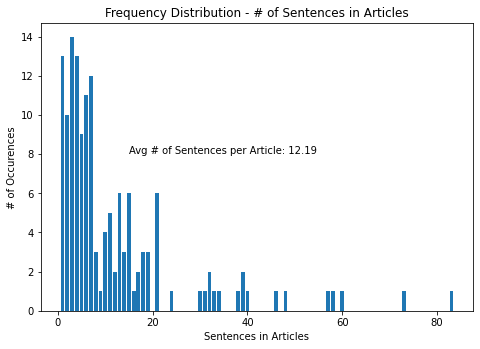
\includegraphics[width = 400pt]{Images/sentences_per_article.png}
            \caption{Distribution of Sentence Count per Article}
            \end{figure}
            
            \begin{table}[H]
            \centering
            \resizebox{\textwidth}{!}{%
            \begin{tabular}{|l|ll|ll|ll|ll|}
            \hline
            \textbf{Batch Size} &
              \multicolumn{2}{c|}{\textbf{X-Small}} &
              \multicolumn{2}{c|}{\textbf{Small}} &
              \multicolumn{2}{c|}{\textbf{Medium}} &
              \multicolumn{2}{c|}{\textbf{Large}} \\ \hline
            \textbf{Set} &
              \textbf{Train} &
              \textbf{Test} &
              \textbf{Train} &
              \textbf{Test} &
              \textbf{Train} &
              \textbf{Test} &
              \textbf{Train} &
              \textbf{Test} \\ \hline
            \# of Articles  & 5 & 140 & 9 & 136 & 23 & 122 & 45 & 100 \\
            \# of Sentences & 49.6 & 1,718.4 & 100.6 & 1,667.4 & 246.3 & 1,521.7 & 505.8 & 1,262.2 \\
            \# of Non-Entities & 841.2 & 31,734.8 & 1,753.1 & 30,822.9 & 4,380.9 & 28,195.1 & 9,321.7 & 23,254.3 \\
            \# of Entities  & 181.1 & 6,249.9 & 406.6 & 6,024.4 & 972.2 & 5,458.8 & 2,018.7 & 4,412.3 \\ \hline
            \end{tabular}%
            }
            \caption{Metrics by Training Test Split}{(Averaged over 10 Randomized Replications)}
            \label{tab:my-table}
            \end{table}
            
    \newpage
            
    \begin{comment}
    \section{Entity Weighting Shortcomings}
        While there are parameters in model generation that could theoretically "brute force" specific named entities into the output, doing so tended to hinder generation as it would impact the models confidence in a trade-off to ensure the token was included. Furthermore, support for this parameter is currently removed. Other approaches to giving more weight towards entities or other "keywords" have been taken, but require tweaking the underlying transformer structure.
        
        One such approach attempts to utilize keywords from the source document as a way to provide clues on what is important for the model. The encoder (a BiLSTM) reads in both the input sentence and a list of keywords taken from said input sentence, at which point a separate keyword extractor determines if the items in the list are actually important contextually. Then, the information from the original sentence and the classified keywords is analyzed via dual-attention to generate a context vector which is fed into the decoder.
        
        Another method follows a similar route, in that during the encoding stage a notion of "word importance" is applied to the inputs. This is applied in two ways. The first approach is applied through TF-IDF scoring, which stands for "term frequency-inverse document frequency" and acts as a statistical metric that evaluates how relevant a word is in the context of a source document. The second approach focuses on modifying the attention scoring mechanism through the use of learned weightings while encoding. The results of this approach were inconclusive, as the original baseline testing was not found to be as expected when compared to other state-of-the-art methods and thus any improvement over said baseline was not reliable.
        
        %https://ojs.aaai.org/index.php/AAAI/article/view/6333/6189
        %https://web.stanford.edu/class/archive/cs/cs224n/cs224n.1174/reports/2762071.pdf
    \end{comment}
    
    
    \section{Data Augmentation Method Results}
            \subsubsection{Linearization}
                Attempts to linearize entity tags into the sentence prior to summarization resulted in a high degree of incoherency (wherein the model did not know how to interpret the linearized tags in a summary). As a result, linearization was unsuccessful.
                
            \subsubsection{Named Entity Weighting \& Stemming}
                While in theory weighting named entities to the front of the articles should produce a generation output with a higher number of entities due to how models are trained, this only resulted in one viable generated output. As for stemming, nearly all articles contained a sufficient number of entities within each sentence and as a result would have rarely removed sentences. Furthermore, the generated output from a shuffle post-stem often did not vary from the original un-stemmed version if the sentence removed were to be replaced back in the proper location. As a result, this approach was passed on in favour of the simpler shuffling mechanic.
    
    \section{NER Model Settings}
        Training settings for the BERT-Base Cased model iterated through 3 epochs with a learning rate of 2e-5 (0.00002) and a weight decay rate of 0.01. The model was evaluated with Precision, Recall, and F1 metrics.


    \newpage
    \section{Model Results}
        Table \ref{tab:results} below illustrates precision, recall, and F1 metrics on the testing set when the model was trained via their respective training sets. Training was randomized and was replicated 10 times on different train-test variations of the same batch-size to provide an accurate confidence interval on the accuracy metrics.
        
        To make results clearer, the dataset with the highest F1 score for each batch size is bolded. The original dataset pertains to a batch of un-augmented data. In the case of the baseline datasets (Rules and Paraphrased), they contain the original un-augmented data and an additional three augmented sentences per original sentence. In the case of the summarization methods (Article, One Tag, and Uni Tag, as seen in Table 4.2), they contain the original un-augmented data and then take a number of generated summaries that is equal to three times the number of sentences in the original article to approximately match the three additions from the baseline (as each generated summary is often one sentence).
        
        The metrics for the Rules dataset are for the highest-performing \\method/binomial rate combination (LWTR at a rate of 10\%), though results across methods within rates were quite similar. As the rate increased, performance dropped slightly across all rule-based methods.
        \\\\
        Overall, we see that the Rules based data augmentation method performed the best by a sizeable amount, with paraphrased and article augmentation methods falling slightly behind. One key difference is that the rules-based approach tends to have a significantly higher recall score at low batch sizes than the other two methods, which contributes to the higher F1 score overall as in comparison precision is quite similar albeit also somewhat higher.
        
        \begin{table}[H]
        \begin{center}
        \begin{tabular}{|c|l|lll|}
        \hline
        \textbf{Batch Size} & \multicolumn{1}{c|}{\textbf{Dataset}} & \multicolumn{1}{c}{\textbf{Precision}} & \multicolumn{1}{c|}{\textbf{Recall}} & \multicolumn{1}{c|}{\textbf{F1-Score}} \\ \hline
        \multirow{6}{*}{\begin{tabular}[c]{@{}c@{}}\textbf{X-Small}\\(S=50)\end{tabular}}
         & Original & 3.33\%$\pm$6.53\% & \multicolumn{1}{l|}{0.00\%$\pm$0.00\%} & 0.01\%$\pm$0.01\% \\
         & \textbf{Rules*} & \textbf{26.28\%$\pm$ 7.18\%} & \multicolumn{1}{l|}{\textbf{16.48\%$\pm$ 4.79\%}} & \textbf{20.01\%$\pm$ 5.16\%} \\
         & Paraphrased & 22.38\%$\pm$ 6.27\% & \multicolumn{1}{l|}{8.37\%$\pm$ 3.08} & 11.68\%$\pm$ 3.56\% \\
         & Article & 23.46\%$\pm$ 5.98\% & \multicolumn{1}{l|}{8.69\%$\pm$ 3.65\%} & 12.05\%$\pm$ 4.41\% \\
         & One Tag & 15.97\%$\pm$ 9.63\% & \multicolumn{1}{l|}{0.91\%$\pm$ 0.88\%} & 1.64\%$\pm$ 1.56\% \\
         & Uni Tag & 16.38\%$\pm$ 9.10\% & \multicolumn{1}{l|}{1.83\%$\pm$ 1.47\%} & 3.06\%$\pm$ 2.33\% \\ \hline
         \multirow{6}{*}{\begin{tabular}[c]{@{}c@{}}\textbf{Small}\\(S=100)\end{tabular}}
         & Original & 8.45\%$\pm$5.56\% & \multicolumn{1}{l|}{0.59\%$\pm$0.77\%} & 0.99\%$\pm$1.23\% \\
         & \textbf{Rules*} & \textbf{53.77\%$\pm$ 3.1\%} & \multicolumn{1}{l|}{\textbf{59.14\%$\pm$ 7.34\%}} & \textbf{56.18\%$\pm$ 4.84\%} \\
         & Paraphrased & 47.27\%$\pm$ 2.58\% & \multicolumn{1}{l|}{47.64\%$\pm$ 5.06} & 47.20\%$\pm$ 3.75\% \\
         & Article & 43.49\%$\pm$ 3.83\% & \multicolumn{1}{l|}{40.2\%$\pm$ 5.62\%} & 41.61\%$\pm$ 4.71\% \\
         & One Tag & 23.18\%$\pm$ 3.07\% & \multicolumn{1}{l|}{12.56\%$\pm$ 3.37\%} & 16.03\%$\pm$ 3.47\% \\
         & Uni Tag & 25.32\%$\pm$ 2.35\% & \multicolumn{1}{l|}{15.52\%$\pm$ 3.33\%} & 18.91\%$\pm$ 3.12\% \\ \hline
         \multirow{6}{*}{\begin{tabular}[c]{@{}c@{}}\textbf{Medium}\\(S=250)\end{tabular}}
         & Original & 41.52\%$\pm$2.97\% & \multicolumn{1}{l|}{42.10\%$\pm$3.90\%} & 41.76\%$\pm$3.32\% \\
         & \textbf{Rules*} & \textbf{70.07\%$\pm$ 1.7\%} & \multicolumn{1}{l|}{\textbf{75.77\%$\pm$ 1.9\%}} & \textbf{72.8\%$\pm$ 1.54\%} \\
         & Paraphrased & 67.34\%$\pm$ 1.03\% & \multicolumn{1}{l|}{69.51\%$\pm$ 2.02} & 68.38\%$\pm$ 1.32\% \\
         & Article & 66.50\%$\pm$ 1.20\% & \multicolumn{1}{l|}{66.34\%$\pm$ 1.66\%} & 66.41\%$\pm$ 1.34\% \\
         & One Tag & 56.21\%$\pm$ 1.53\% & \multicolumn{1}{l|}{47.97\%$\pm$ 2.70\%} & 51.72\%$\pm$ 2.18\% \\
         & Uni Tag & 56.70\%$\pm$ 2.34\% & \multicolumn{1}{l|}{49.23\%$\pm$ 3.24\%} & 52.68\%$\pm$ 2.84\% \\ \hline
         \multirow{6}{*}{\begin{tabular}[c]{@{}c@{}}\textbf{Large}\\(S=500)\end{tabular}}
         & Original & 65.93\%$\pm$1.05\% & \multicolumn{1}{l|}{70.49\%$\pm$1.45\%} & 68.11\%$\pm$0.83\% \\
         & \textbf{Rules*} & \textbf{75.91\%$\pm$ 1.76\%} & \multicolumn{1}{l|}{\textbf{82.19\%$\pm$ 1.21\%}} & \textbf{78.92\%$\pm$ 1.34\%} \\
         & Paraphrased & 74.41\%$\pm$ 1.20\% & \multicolumn{1}{l|}{79.14\%$\pm$ 0.85} & 76.70\%$\pm$ 0.99\% \\
         & Article & 72.75\%$\pm$ 0.84\% & \multicolumn{1}{l|}{75.92\%$\pm$ 0.47\%} & 74.30\%$\pm$ 0.63\% \\
         & One Tag & 68.58\%$\pm$ 1.02\% & \multicolumn{1}{l|}{67.45\%$\pm$ 1.25\%} & 68.00\%$\pm$ 0.96\% \\
         & Uni Tag & 69.96\%$\pm$ 0.88\% & \multicolumn{1}{l|}{69.91\%$\pm$ 1.40\%} & 69.91\%$\pm$ 0.94\% \\ \hline
        \end{tabular}
        \caption{Model Results for Tested Methods ($\alpha$ = 0.05, n=10)}{*\textit{Label-Wise Token Replacement, 10\% Rate}}
        \label{tab:results}
        \end{center}
        \end{table}


\newpage





\chapter{Future Work \\and Conclusions}
    \section{Future Work}
    \subsubsection{Theoretical Optimal Tuning}
        With all the aforementioned uncertainty in summary generation, the process of fine-tuning hyper-parameters would be incredibly costly and time-consuming. The approach that could be taken is discussed in this section, but was not done in actuality.
            
        There are three main hurdles that would require various configurations to be tested to determine the optimal hyper-parameters for ideal summary generation.
        
        \begin{enumerate}
            \item \textbf{Model Hyper-Parameters:} As discussed in the previous sections, there are a large number of model parameters that can be adjusted to tweak generated outputs. In total, there are seven parameters of interest that would need to be tested, these being: search method (greedy or beam), sampling type (top-k or top-p), temperature, repetition penalty, and minimum length.
            \item \textbf{Article Variations:} Also discussed prior, the four variations on the original articles that intend to make generation easier for the model would all need to be evaluated.
            \item \textbf{Shuffle Variations:} Lastly, different shuffling of article sentences would need to be tested for further consistency.
        \end{enumerate}
        
        These variations would then have to be examined by human eye, though ROUGE filtering could help cut down manual labour required. Overall, combining the three core factors that would need to be tested rigorously results in a theoretical number of combinations too costly to examine. For instance, examining 30 shuffled variants across the 4 article variations takes upwards of 12 hours on one set of conservative model hyper-parameters. As such, configuring all 7 and trying various combinations in a grid-search method would take many days.
    
    \subsubsection{Higher Augment Multiples}
        While the paraphrasing and abstractive summarization results are fairly similar, there is a limit to how many paraphrased variations models can generate. While the sentence "His name was Bill Gates and he founded Microsoft" could viably be paraphrased in three other ways (e.g. "Named Bill Gates, he is the founder of Microsoft, etc.), results are often still quite similar and not varied. With this in mind, it would be worth exploring the impact of (a) a higher augment multiple (i.e. augment 7 new sentences instead of 3 from one original) and (b) how paraphrasing holds up against summarization in these scenarios.
    
\section{Project Conclusion}
    
    \subsubsection{The Aim}
    The goal of this project was to explore a new method of data augmentation specifically for the natural language processing task of tagging named entities. Current methods of data augmentation for NER tasks include simple algorithmic rules-based approaches, as well as more complicated generational approaches such as back-translation, paraphrasing, and sequential generation. As a new approach, abstractive summarization was explored and tested.
    
    \subsubsection{Methods Explored}
    With the new approach via abstractive summarization, some unique challenges presented themselves. Firstly, generating a summary requires sentences that are related to one another and pertain to the same context. Furthermore, a single sentence cluster (article) will only generate one to two sentences at most, meaning that an article that is 40 sentences in length will only have 2 new augmented sentences. However, human generated summaries tend to be constructed from the first few sentences of an article; as a result, models that are focused on generating summaries (PEGASUS) tend to have inherently learned a higher weighting for the initial sentences in longer articles. With this in mind, we can shuffle the sentences within an article to significantly alter the generated summary output. Through this technique, the article with 40 sentences can now be re-shuffled many times to provide as many augmented sentences as necessary.
    
    Summary generation is not always consistent; in an attempt to increase consistency, methods of replacing entities with their associated tags (somewhat similar to sentence linearization) prior to generation were also explored.
    
    \subsubsection{Conclusion}
    The results of summary generation with and without tag replacement were significantly lower for all batch sizes, with the tag replaced variants performing much worse on lower sample sizes. As for the original article summary method without tags replaced, it performed only slightly worse to the paraphrasing method performed in other research. Though it did outperform on the smallest batch size, this could simply be due to only 10 replications being performed. When compared to the rules-based approach baseline however, both the paraphrasing method and abstractive summarization techniques end up being outperformed by a fairly significant margin at the X-Small, Small, and Medium batch sizes. At the large batch size, all methods provide a slight boost but are much closer in performance.





\clearpage
\addtocounter{chapter}{1}
\addcontentsline{toc}{chapter}{\protect\numberline{\thechapter} Bibliography}

\begin{thebibliography}{9}

    \bibitem{Rules}
        Xiang Dai and Heike Adel. (2020) \emph{An Analysis of Simple Data Augmentation for Named Entity Recognition}.
        https://aclanthology.org/2020.coling-main.343.pdf
    
    \bibitem{Gen}
        Bosheng Ding, Linlin Liu, Lidong Bing, Canasai Kruengkrai, Thien Hai Nguyen, Shafiq Joty, Luo Si, and Chunyan Miao. (2020) \emph{DAGA: Data Augmentation with a Generation Approach for Low-resource Tagging Tasks}.
        https://aclanthology.org/2020.emnlp-main.488.pdf
    
    \bibitem{Cross}
        Shuguang Chen, Gustavo Aguilar, Leonardo Neves, and Thamar Solorio. (2021) \emph{Data Augmentation for Cross-Domain Named Entity Recognition}.
        https://arxiv.org/pdf/2109.01758.pdf
    
    \bibitem{Back}
        Usama Yaseen and Stefan Langer. (2021) \emph{Data Augmentation for Low-Resource Named Entity Recognition Using Backtranslation}.
        https://arxiv.org/pdf/2108.11703v1.pdf
    
    \bibitem{Sum}
        Petr Marek, Štěpán Müller, Jakub Konrád, Petr Lorenc, Jan Pichl, and Jan Šedivý. (2021) \emph{Text Summarization of Czech News Articles Using Named Entities}.
        https://arxiv.org/pdf/2104.10454.pdf
    
    \bibitem{RoBERTA}
        Yinhan Liu, Myle Ott, Naman Goyal, Jingfei Du, Mandar Joshi, Danqi Chen, Omer Levy, Mike Lewis, Luke Zettlemoyer, and Veselin Stoyanov. (2019) \emph{RoBERTa: A Robustly Optimized BERT Pretraining Approach}.
        https://arxiv.org/abs/1907.11692
    
    \bibitem{BART}
        Mike Lewis, Yinhan Liu, Naman Goyal, Marjan Ghazvininejad, Abdelrahman Mohamed, Omer Levy, Ves Stoyanov, and Luke Zettlemoyer. (2019) \emph{BART: Denoising Sequence-to-Sequence Pre-training for Natural Language Generation, Translation, and Comprehension}.
        https://arxiv.org/abs/1910.13461

    \bibitem{Marian}
        Marcin Junczys-Dowmunt, Roman Grundkiewicz, Tomasz Dwojak, Hieu Hoang, Kenneth Heafield, Tom Neckermann, Frank Seide, Ulrich Germann, Alham Fikri Aji, Nikolay Bogoychev, André F. T. Martins, and Alexandra Birch. (2018) \emph{Marian: Fast Neural Machine Translation in C++}.
        https://arxiv.org/abs/1804.00344 

    \bibitem{T5}
        Colin Raffel, Noam Shazeer, Adam Roberts, Katherine Lee, Sharan Narang, Michael Matena, Yanqi Zhou, Wei Li, and Peter J. Liu. (2019) \emph{Exploring the Limits of Transfer Learning with a Unified Text-to-Text Transformer}.
        https://arxiv.org/abs/1910.10683
        
    \bibitem{GPT2}
        OpenAI (2019) \emph{GPT-2: 1.5B Release}
        https://openai.com/blog/tags/gpt-2/
        
        
        
    \bibitem{PEGASUS}
        Jingqing Zhang, Yao Zhao, Mohammad Saleh and Peter J. Liu (2020) \emph{PEGASUS: Pre-training with Extracted Gap-sentences for Abstractive Summarization}
        https://arxiv.org/pdf/1912.08777.pdf
        
    
    \bibitem{BERT}
        Jacob Devlin, Ming-Wei Chang, Kenton Lee and Kristina Toutanova (2019) \emph{BERT: Pre-training of Deep Bidirectional Transformers for Language Understanding}
        https://arxiv.org/pdf/1810.04805.pdf
        
        
        
    \bibitem{Paraphrasing}
        Rui Wang and Ricardo Henao (2021) \emph{Unsupervised Paraphrasing Consistency Training for Low Resource
Named Entity Recognition}.
        https://aclanthology.org/2021.emnlp-main.430.pdf
    
    \bibitem{Degen}
        Ari Holtzman, Jan Buys, Li Du, Maxwell Forbes, and Yejin Choi (2020) \emph{THE CURIOUS CASE OF NEURAL TEXT DeGENERATION}
        https://arxiv.org/pdf/1904.09751.pdf
    
    \bibitem{Anon}
        Anonymous Authors (2020) \emph{NEURAL TEXT DEGENERATION WITH UNLIKELIHOOD TRAINING}
    https://openreview.net/attachment?id=SJeYe0NtvH\&name=original\_pdf
    
    \bibitem{unlik}
        Pranav Ajit Nair and Anil Kumar Singh (2021) \emph{On Reducing Repetition in Abstractive Summarization}
        https://aclanthology.org/2021.ranlp-srw.18.pdf
    
    \bibitem{hallucinate}
        Feng Nan, Ramesh Nallapati, Zhiguo Wang, Cicero Nogueira dos Santos, Henghui Zhu, Dejiao Zhang, Kathleen McKeown and Bing Xiang (2021)\emph{Entity-level Factual Consistency of Abstractive Text Summarization}
        https://arxiv.org/pdf/2102.09130.pdf
    
    \bibitem{HF}
        Patrick Von Platen (2020, March 18). \emph{How to generate text: using different decoding methods for language generation with Transformers} HuggingFace.
        https://huggingface.co/blog/how-to-generate
    
    \bibitem{data_source}
        Pritish Uplavikar (2016). \emph{Named Entity Recognition, Wikigold CONLL}
        https://github.com/pritishuplavikar/Named-Entity-Recognition/blob/master/wikigold.conll.txt
    
    \bibitem{HF_course}
        HuggingFace. \emph{How do Transformers Work?}
        https://huggingface.co/course/chapter1/4?fw=pt
    
\end{thebibliography}



\chapter{Appendices} %Use \chapter*{} to hide numbering/from TOC
    \section{Code Files}
    \textbf{Note:} Files are not fully integrate-able in an automated manner. Functions were run in an IDE and thus utilized pre-declared variables that would otherwise be unknown due to not being fed as a function input (e.g. "df").
        \subsection{Main Code Files}
            \subsubsection{Summarization/Paraphrase Model}
                \lstinputlisting[language=Python]{Python/Summarizations\_V2.py}
                \newpage
            \subsubsection{NER Model}
                \lstinputlisting[language=Python]{Python/NER.py}
                \newpage
            \subsubsection{Baseline Augmenting}
                \lstinputlisting[language=Python]{Python/Baseline\_Methods.py}
                \newpage
            \subsubsection{Mapping Functions}
                \lstinputlisting[language=Python]{Python/Mappings.py}
                \newpage
            
        \subsection{Secondary Code Files}
            \subsubsection{Dataset Statistics}
                \lstinputlisting[language=Python]{Python/Dataset\_Statistics.py}
                \newpage
            \subsubsection{Train-Test Split}
                \lstinputlisting[language=Python]{Python/Train\_Test\_RNG\_Splitter.py}
        




\end{document}